%%%%%%%%%%%%%%%%%%%%%%%%%%%%%%%%%%%%%%%%%
% Beamer Presentation
% LaTeX Template
% Version 1.0 (10/11/12)
%
% This template has been downloaded from:
% http://www.LaTeXTemplates.com
%
% License:
% CC BY-NC-SA 3.0 (http://creativecommons.org/licenses/by-nc-sa/3.0/)
%
%%%%%%%%%%%%%%%%%%%%%%%%%%%%%%%%%%%%%%%%%

%----------------------------------------------------------------------------------------
%    PACKAGES AND THEMES
%----------------------------------------------------------------------------------------

\documentclass{beamer}
\newcommand{\bx}{\mathbf{x}}
\newcommand{\ii}{\mathrm{i}}
\newcommand{\bxi}{\bm{\xi}}
\newcommand{\bmu}{\bm{\mu}}
\newcommand{\bb}{\mathbf{b}}
\newcommand{\bA}{\mathbf{A}}
\newcommand{\bJ}{\mathbf{J}}
\newcommand{\bB}{\mathbf{B}}
\newcommand{\bM}{\mathbf{M}}

\newcommand{\by}{\mathbf{y}}
\newcommand{\bw}{\mathbf{w}}

\newcommand{\bX}{\mathbf{X}}
\newcommand{\bY}{\mathbf{Y}}
\newcommand{\bs}{\mathbf{s}}
\newcommand{\sign}{\mathrm{sign}}
\newcommand{\bt}[0]{\bm{\theta}}
\newcommand{\bc}{\mathbf{c}}
\newcommand{\bzero}{\mathbf{0}}
\renewcommand{\bf}{\mathbf{f}}
\newcommand{\bu}{\mathbf{u}}
\newcommand{\bv}[0]{\mathbf{v}}
\mode<presentation> {

% The Beamer class comes with a number of default slide themes
% which change the colors and layouts of slides. Below this is a list
% of all the themes, uncomment each in turn to see what they look like.

%\usetheme{default}
%\usetheme{AnnArbor}
%\usetheme{Antibes}
%\usetheme{Bergen}
%\usetheme{Berkeley}
%\usetheme{Berlin}
%\usetheme{Boadilla}
%\usetheme{CambridgeUS}
%\usetheme{Copenhagen}
%\usetheme{Darmstadt}
%\usetheme{Dresden}
%\usetheme{Frankfurt}
%\usetheme{Goettingen}
%\usetheme{Hannover}
%\usetheme{Ilmenau}
%\usetheme{JuanLesPins}
%\usetheme{Luebeck}
\usetheme{Madrid}
%\usetheme{Malmoe}
%\usetheme{Marburg}
%\usetheme{Montpellier}
%\usetheme{PaloAlto}
%\usetheme{Pittsburgh}
%\usetheme{Rochester}
%\usetheme{Singapore}
%\usetheme{Szeged}
%\usetheme{Warsaw}


% As well as themes, the Beamer class has a number of color themes
% for any slide theme. Uncomment each of these in turn to see how it
% changes the colors of your current slide theme.

%\usecolortheme{albatross}
\usecolortheme{beaver}
%\usecolortheme{beetle}
%\usecolortheme{crane}
%\usecolortheme{dolphin}
%\usecolortheme{dove}
%\usecolortheme{fly}
%\usecolortheme{lily}
%\usecolortheme{orchid}
%\usecolortheme{rose}
%\usecolortheme{seagull}
%\usecolortheme{seahorse}
%\usecolortheme{whale}
%\usecolortheme{wolverine}

%\setbeamertemplate{footline} % To remove the footer line in all slides uncomment this line
%\setbeamertemplate{footline}[page number] % To replace the footer line in all slides with a simple slide count uncomment this line

%\setbeamertemplate{navigation symbols}{} % To remove the navigation symbols from the bottom of all slides uncomment this line
}
\usepackage{booktabs}
\usepackage{makecell}
\usepackage{soul}
\newcommand{\red}[1]{\textcolor{red}{#1}}
%
%\usepackage{graphicx} % Allows including images
%\usepackage{booktabs} % Allows the use of \toprule, \midrule and \bottomrule in tables
%
%
%\usepackage{amsthm}
%
%\usepackage{todonotes}
%\usepackage{floatrow}
%
%\usepackage{pgfplots,algorithmic,algorithm}
%\usepackage[toc,page]{appendix}
%\usepackage{float}
%\usepackage{booktabs}
%\usepackage{bm}
%
%\theoremstyle{definition}
%
\newcommand{\RR}[0]{\mathbb{R}}
%
%\newcommand{\bx}{\mathbf{x}}
%\newcommand{\ii}{\mathrm{i}}
%\newcommand{\bxi}{\bm{\xi}}
%\newcommand{\bmu}{\bm{\mu}}
%\newcommand{\bb}{\mathbf{b}}
%\newcommand{\bA}{\mathbf{A}}
%\newcommand{\bJ}{\mathbf{J}}
%\newcommand{\bB}{\mathbf{B}}
%\newcommand{\bM}{\mathbf{M}}
%\newcommand{\bF}{\mathbf{F}}
%
%\newcommand{\by}{\mathbf{y}}
%\newcommand{\bw}{\mathbf{w}}
%\newcommand{\bn}{\mathbf{n}}
%
%\newcommand{\bX}{\mathbf{X}}
%\newcommand{\bY}{\mathbf{Y}}
%\newcommand{\bs}{\mathbf{s}}
%\newcommand{\sign}{\mathrm{sign}}
%\newcommand{\bt}[0]{\bm{\theta}}
%\newcommand{\bc}{\mathbf{c}}
%\newcommand{\bzero}{\mathbf{0}}
%\renewcommand{\bf}{\mathbf{f}}
%\newcommand{\bu}{\mathbf{u}}
%\newcommand{\bv}[0]{\mathbf{v}}

\AtBeginSection[]
{
   \begin{frame}
       \frametitle{Outline}
       \tableofcontents[currentsection]
   \end{frame}
}

%----------------------------------------------------------------------------------------
%    TITLE PAGE
%----------------------------------------------------------------------------------------
\usepackage{bm}
\newcommand*{\TakeFourierOrnament}[1]{{%
\fontencoding{U}\fontfamily{futs}\selectfont\char#1}}
\newcommand*{\danger}{\TakeFourierOrnament{66}}

\title[ADCME]{ADCME: Automatic Differentiation Library for Computational and Mathematical Engineering} % The short title appears at the bottom of every slide, the full title is only on the title page

\author{\url{https://github.com/kailaix/ADCME.jl}} % Your name
\institute[] % Your institution as it will appear on the bottom of every slide, may be shorthand to save space
{
%ICME, Stanford University \\ % Your institution for the title page
%\medskip
%\textit{kailaix@stanford.edu}\quad \textit{darve@stanford.edu} % Your email address
}
\date{\today} % Date, can be changed to a custom date

% Mathematics of PDEs


\begin{document}

%\usebackgroundtemplate{%
%  \includegraphics[width=\paperwidth,height=\paperheight]{figures/back}} 
\begin{frame}
\titlepage % Print the title page as the first slide

%dfa
\end{frame}


\begin{frame}
	\frametitle{Inverse Modeling}
	\begin{itemize}
		\item \textbf{Inverse modeling} identifies a certain set of parameters or functions with which the outputs of the forward analysis matches the desired result or measurement.
		\item Many real life engineering problems can be formulated as inverse modeling problems: shape optimization for improving the performance of structures, optimal control of fluid dynamic systems, etc.
		\begin{figure}[hbt]
  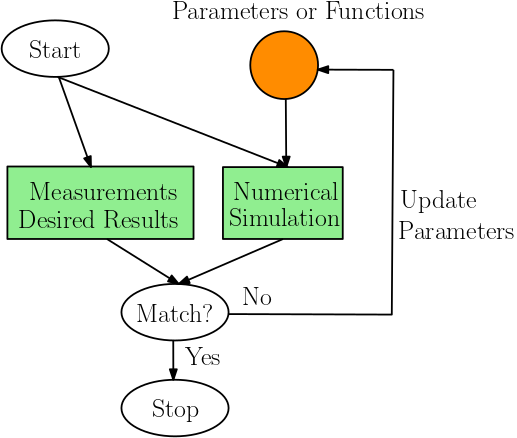
\includegraphics[width=0.4\textwidth]{../im.png}
\end{figure}

	\end{itemize}
\end{frame}

\begin{frame}
	\frametitle{Physics Based Machine Learning}
	\begin{itemize}
		\item Traditional inverse modeling methods utilize efficient numerical schemes and incorporate physical knowledge (first principles); deep learning learns statistical relations from large amounts of training data.
		\item We combine the best of the two worlds and invent \textbf{physics based machine learning}. 
	\end{itemize}
	\begin{figure}[hbt]
  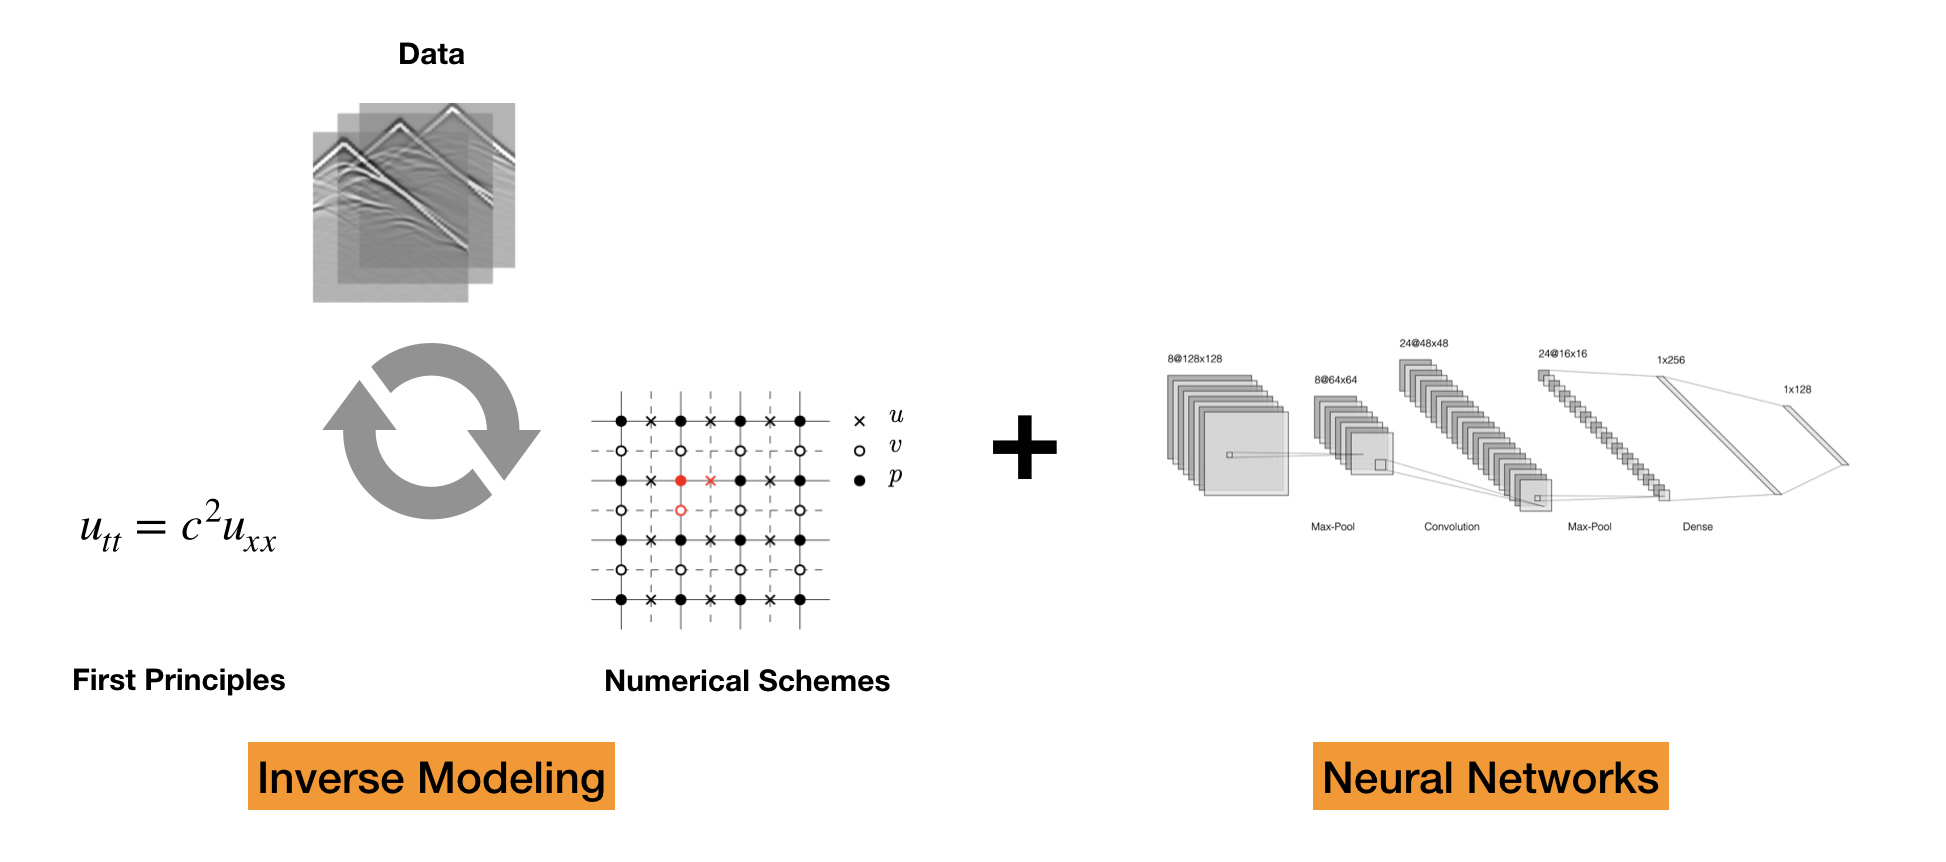
\includegraphics[width=0.9\textwidth]{../physics_based_machine_learning.png}
\end{figure}
\end{frame}

\begin{frame}
	\frametitle{Automatic Differentiation}
	\begin{itemize}
		\item Deep learning and inverse modeling have the same computational model but are disguised under different terminologies.
	\end{itemize}
	\begin{center}
	\small
	\textcolor{red}{
		Back-propagation = Automatic Differentiation = Discrete Adjoint State Method}
	\end{center}
	\begin{figure}[hbt]
  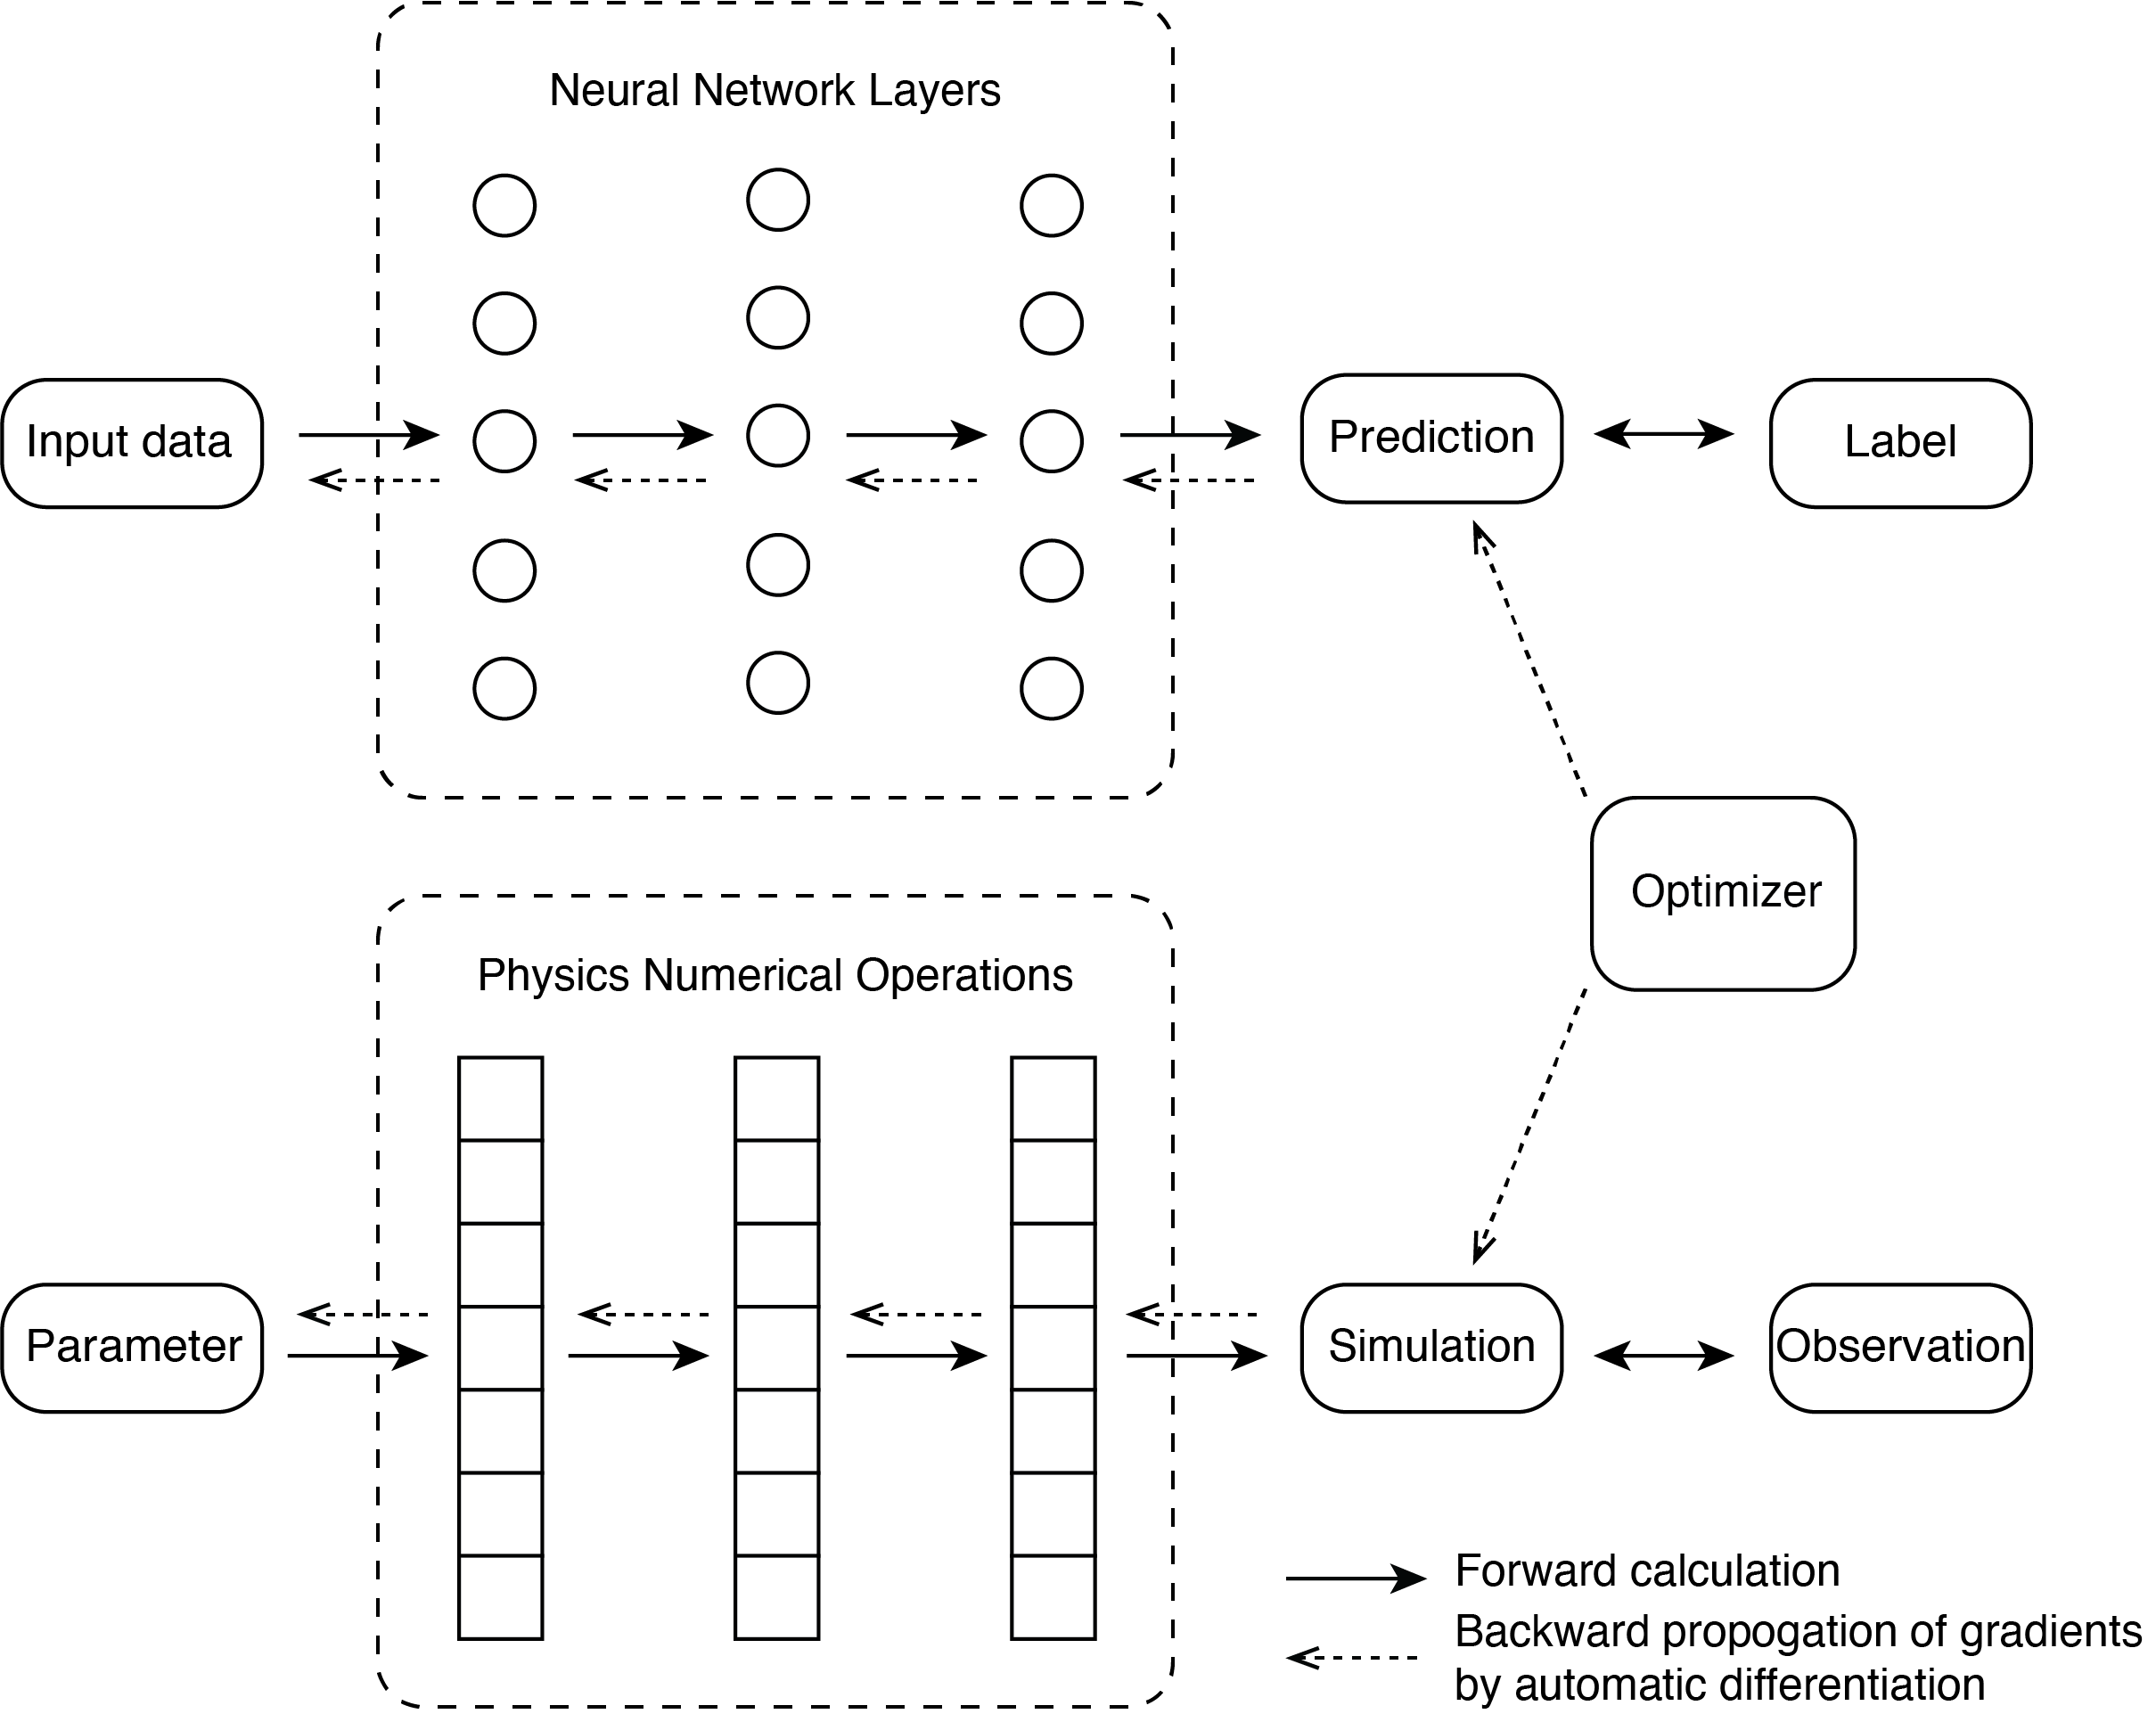
\includegraphics[width=0.6\textwidth]{../compare-NN-PDE.png}
\end{figure}
\end{frame}

\begin{frame}
	\frametitle{AD Implementation in ADCME}
	\begin{itemize}
		\item ADCME allows users to use high level script language Julia to implement numerical simulation codes, but obtain the powerful parallelism and scalability provided by TensorFlow and Julia itself.
		\item Gradients are computed automatically. 
	\end{itemize}
	\begin{figure}[hbt]
  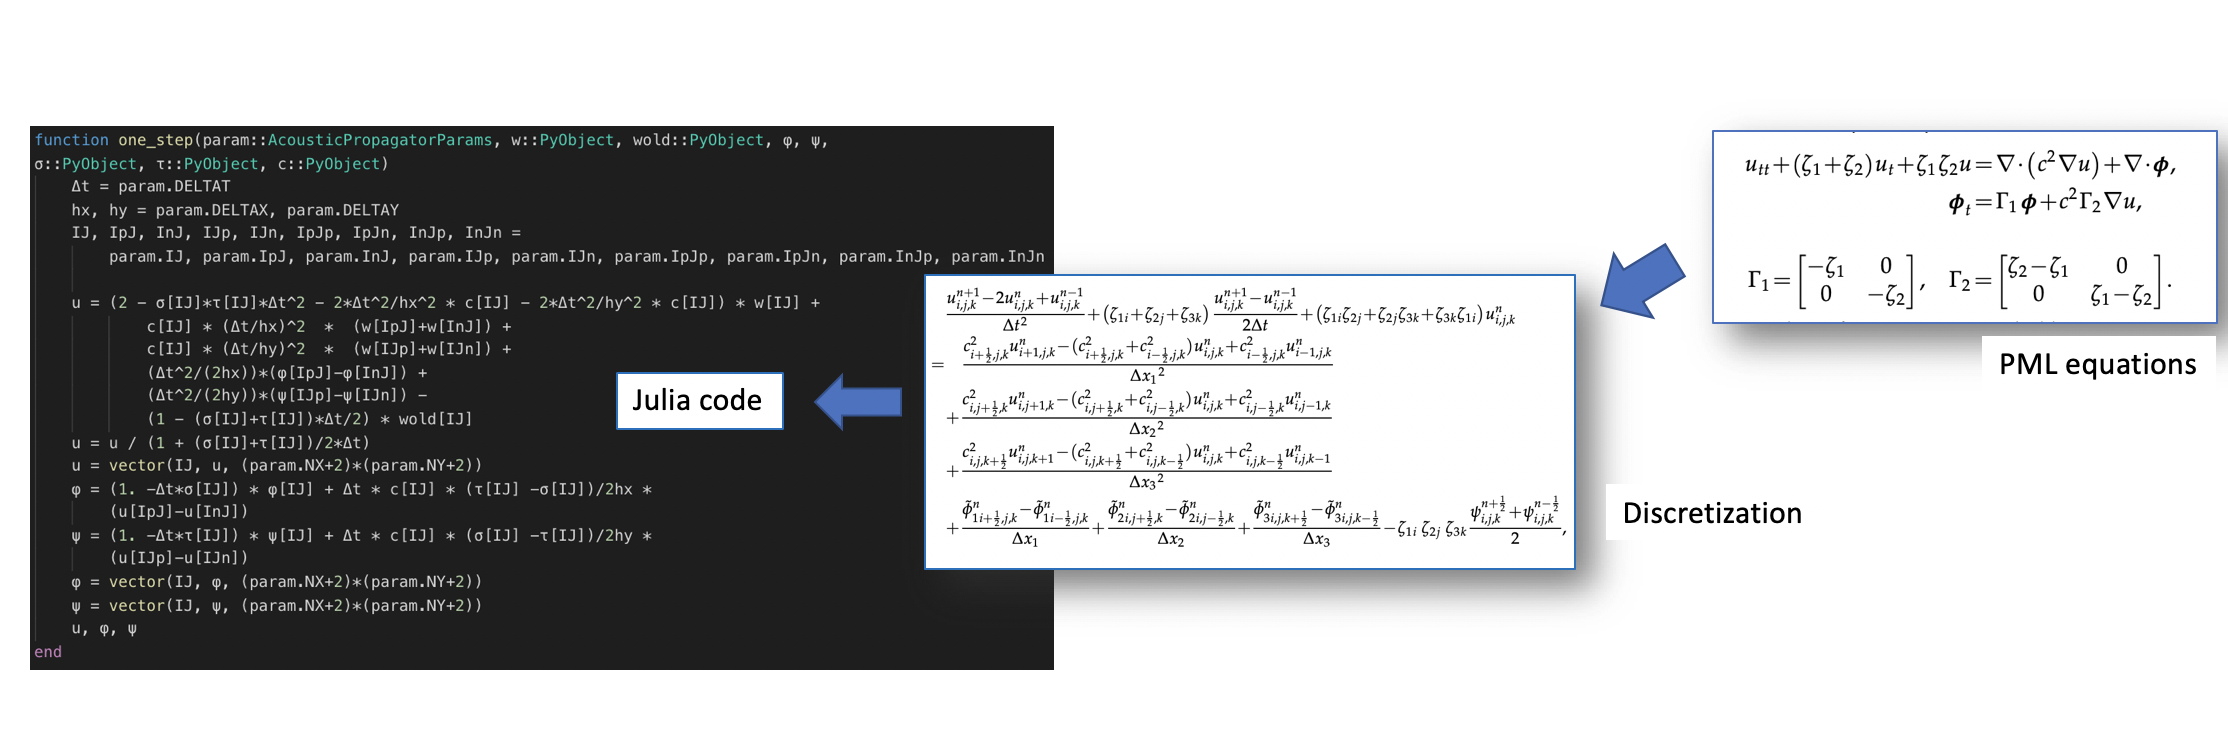
\includegraphics[width=1.0\textwidth]{../Julia.png}
\end{figure}
\end{frame}

\begin{frame}
	\frametitle{Challenges in AD}
	
	
	\begin{minipage}[t]{0.49\textwidth}
	\vspace{-3cm}
\begin{itemize}
	\item ADCME aims to solve the nonlinear implicit operator case via custom operators. 
	\item Another ongoing effort is automatic calculation of Jacobian (\texttt{IGACS.jl}).
\end{itemize}
\end{minipage}~
\begin{minipage}[t]{0.49\textwidth}
  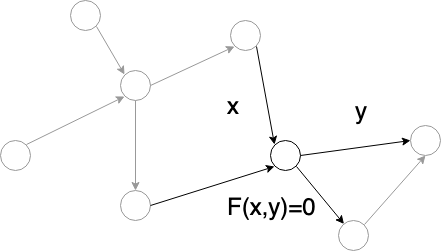
\includegraphics[width=1.0\textwidth]{../sim.png}
\end{minipage}

	% Please add the following required packages to your document preamble:
% \usepackage{booktabs}
\begin{table}[]
\begin{tabular}{@{}lll@{}}
\toprule
Linear/Nonlinear & Explicit/Implicit & Expression   \\ \midrule
Linear           & Explicit          & $y=Ax$       \\
Linear           & Implicit          & $Ax = y$     \\
Nonlinear        & Explicit          & $y = F(x)$   \\
\textbf{Nonlinear}        & \textbf{Implicit}          & $F(x,y) = 0$ \\ \bottomrule
\end{tabular}
\end{table}






\end{frame}

\begin{frame}
	\frametitle{ADCME Solutions}
	% Please add the following required packages to your document preamble:
% \usepackage{booktabs}
\begin{itemize}
	\item Most inverse modeling problems can be classified into 4 categories. For example, the PDE for describing physics is
	\begin{equation}
		\nabla \cdot (\textcolor{red}{X} \nabla u) = 0\quad \mathcal{B}\mathcal{C}(u) = 0
	\end{equation}
	We observe some quantities depending on the solution $u$ and want to estimate $X$.
\end{itemize}
{
\tiny
\begin{table}[]
\begin{tabular}{@{}llll@{}}
\toprule
Expression                                       & Description                & ADCME Solution                         & Note                                     \\ \midrule
$\nabla \cdot (\textcolor{red}{c} \nabla u) = 0$ & Parameter Inverse Problem  & \makecell{Discrete Adjoint\\ State Method}          & Direct optimize the constant $c$                      \\ \hline
$\nabla \cdot (\textcolor{red}{f(x)} \nabla u) = 0$ & Functional Inverse Problem & \makecell{Neural Network \\ Functional Approximator} & $f(x) \approx f_{\theta}(x)$             \\ \hline
$\nabla \cdot (\textcolor{red}{f(u)} \nabla u) = 0$ & Relation Inverse Problem   & \makecell{Deep Learning for\\ Indirect Data}        & $f(u) \approx f_{\theta}(u)$             \\ \hline
$\nabla \cdot (\textcolor{red}{\varpi} \nabla u) = 0$ & Stochastic Inverse Problem & \makecell{Adversarial Numerical\\ Analysis}         & \makecell{Generative Neural Nets for $\varpi$\\ (unknown random processes)} \\ \bottomrule
\end{tabular}
\end{table}
}
\end{frame}


\begin{frame}
	\frametitle{Parameter Inverse Problem: Learning Hidden Geophysical Processes}
	\begin{figure}[hbt]
  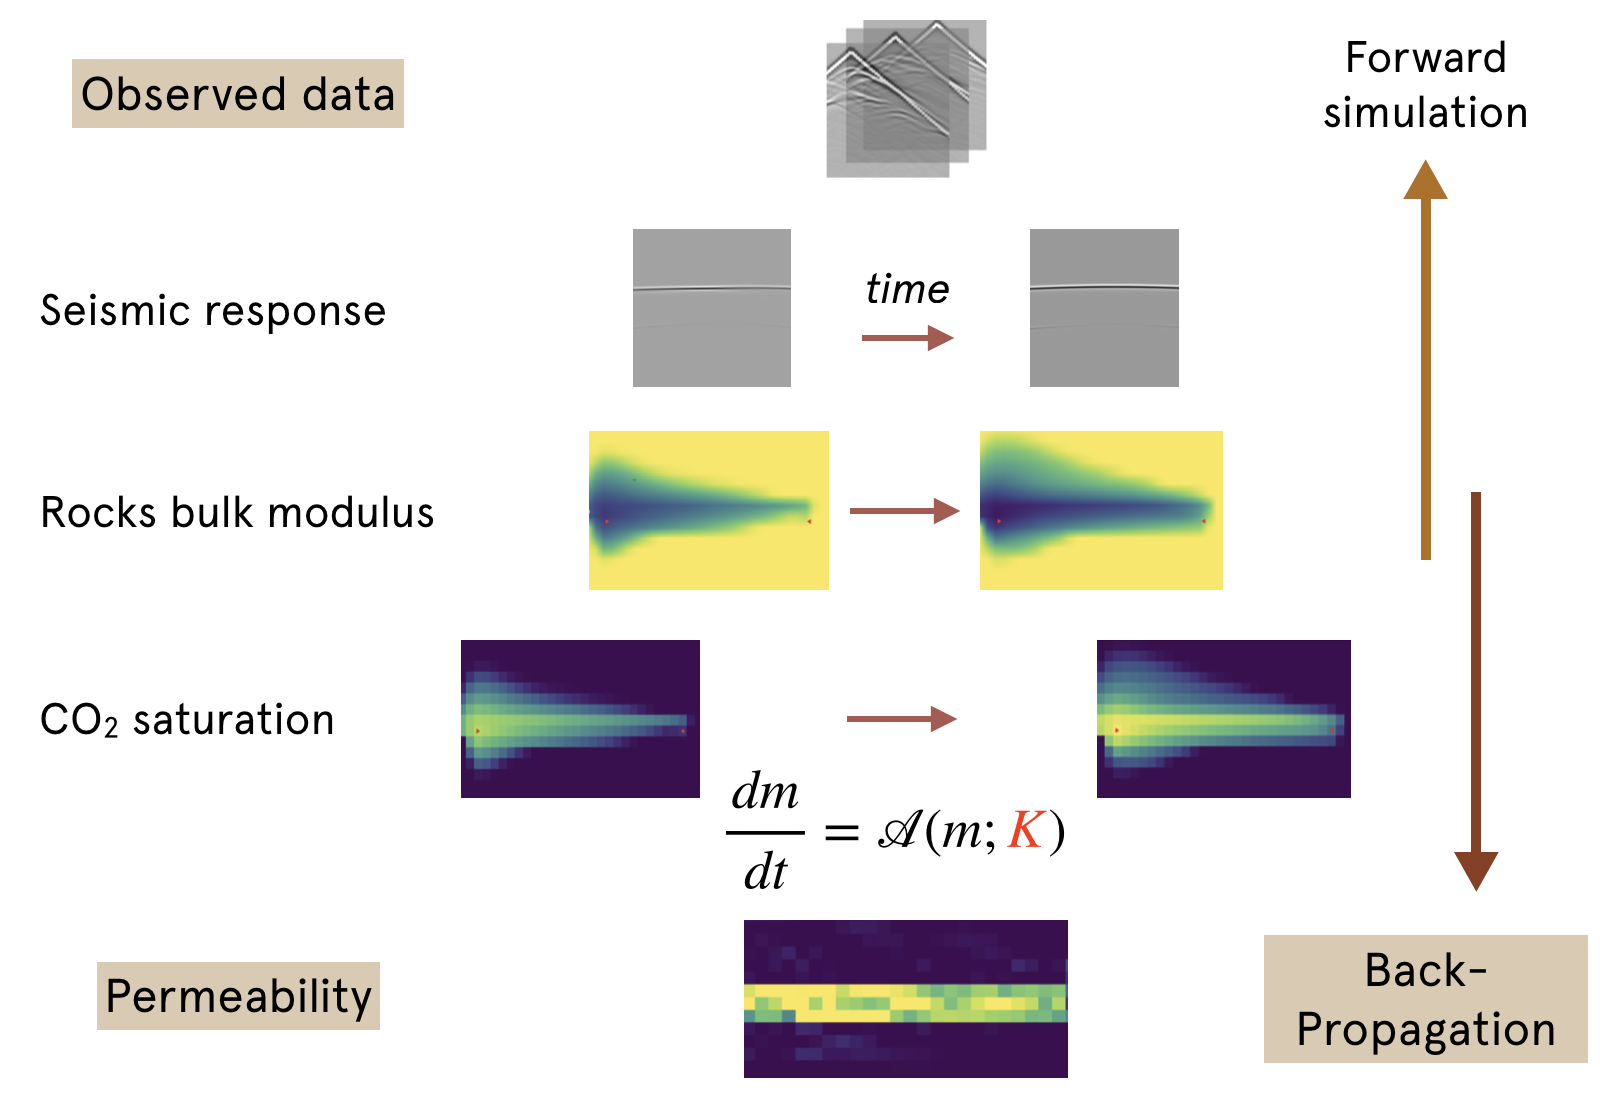
\includegraphics[width=0.8\textwidth]{../geo.png}
\end{figure}
\end{frame}

\begin{frame}
	\frametitle{Functional Inverse Problem: Calibrating L\'evy Processes}
	{\small
	\begin{align*}
		 		& \phi(\bm{\bxi}) = \mathbb{E}[e^{\ii \langle \bxi, \bX_t \rangle}]= \\
		 		& \exp\left[t\left( \ii \langle \bb, \bxi \rangle - \frac{1}{2}\langle \bxi, \bA\bxi\rangle  +\int_{\RR^d} \left( e^{\ii \langle \bxi, \bx\rangle} - 1 - \ii \langle \bxi, \bx\rangle \mathbf{1}_{\|\bx\|\leq 1}\right)\red{\nu(d\bx)}\right) \right]
		 	\end{align*}
		 	}
	\begin{figure}[hbt]
	 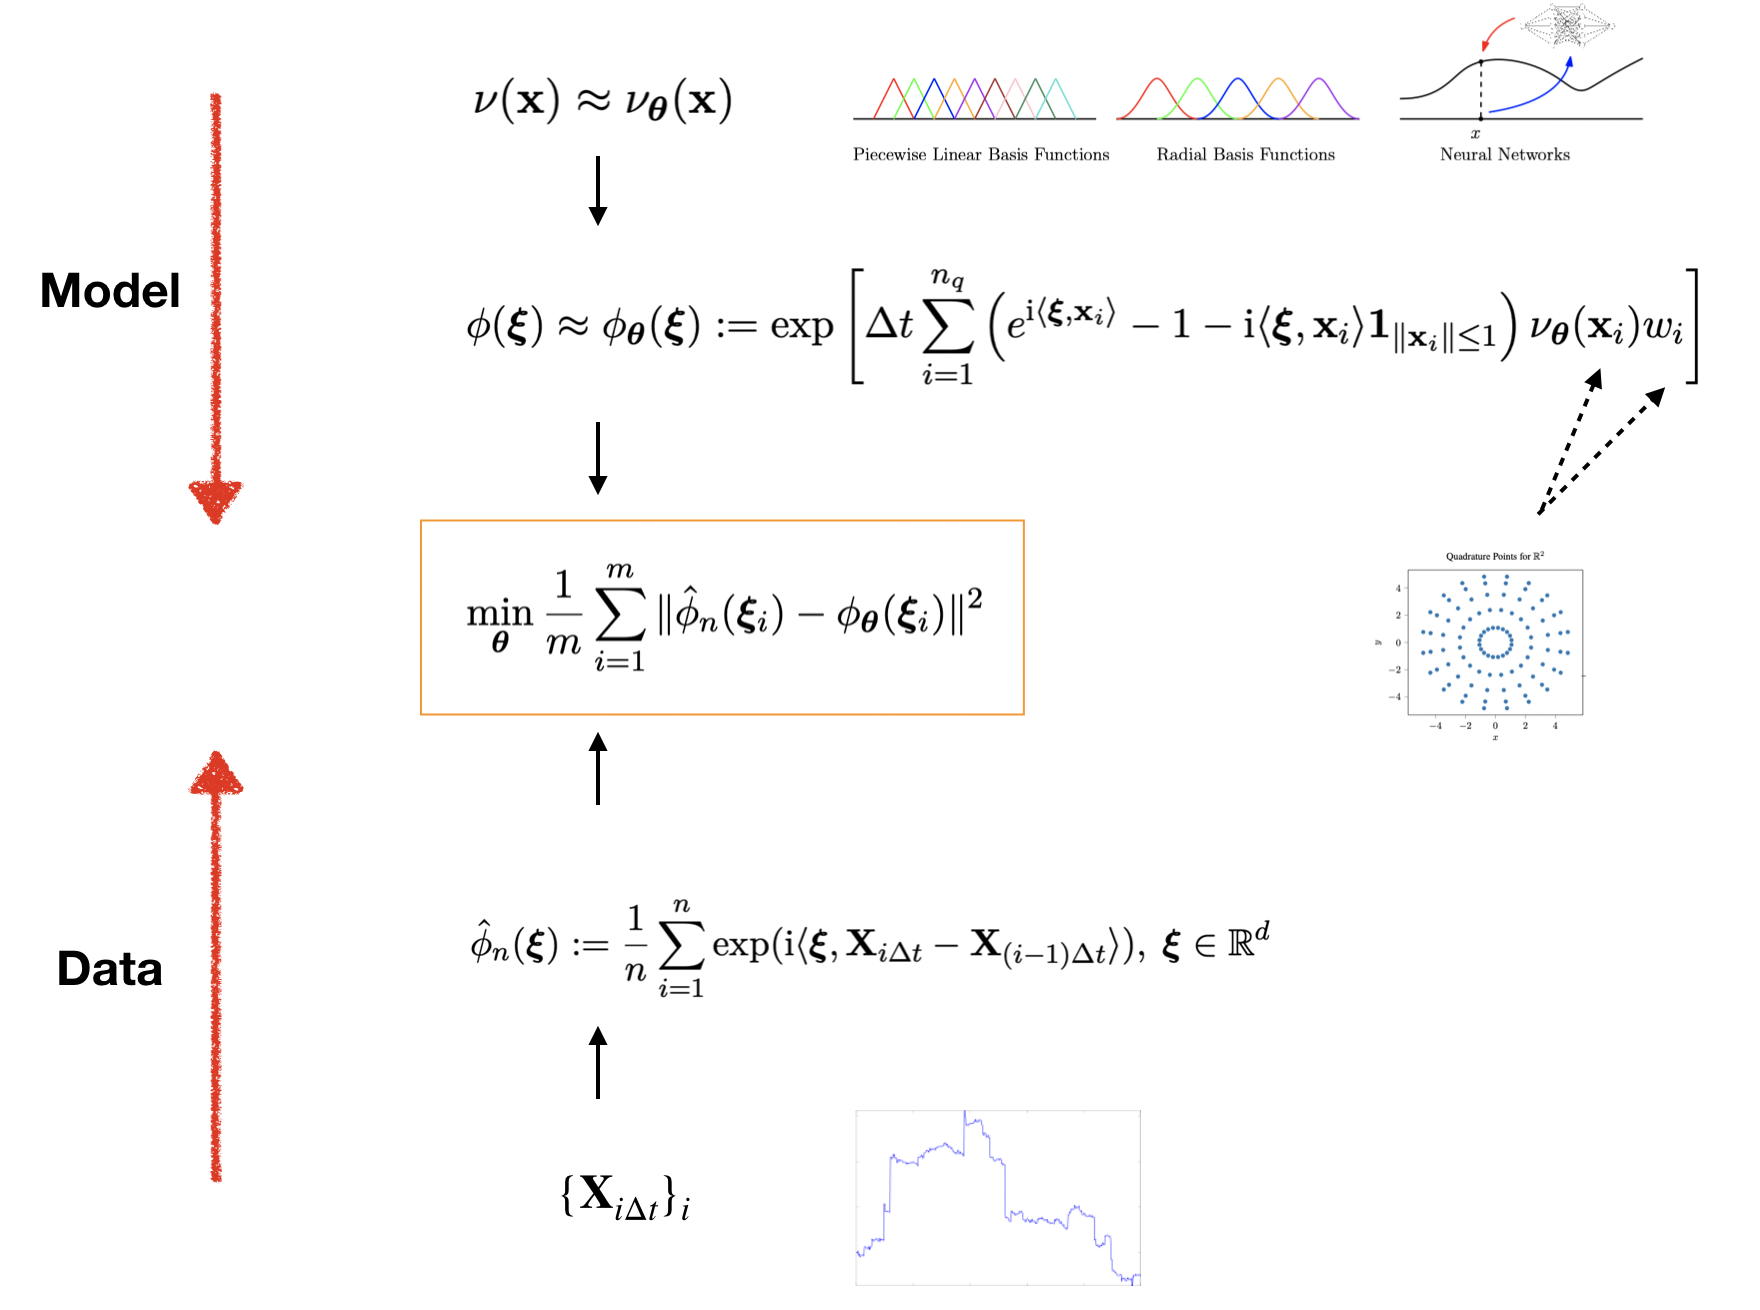
\includegraphics[width=0.6\textwidth]{../algo.png}
\end{figure}
\end{frame}

\begin{frame}
	\frametitle{Relation Inverse Problem: Learning Constitutive Relations}
	\begin{itemize}
		\item Equilibrium equation
		\begin{equation*}
		\mathcal{P}(u(\mathbf{x}), \mathcal{M}(u(\mathbf{x}),\dot u(\mathbf{x}), \mathbf{x})) = \mathcal{F}(u(\mathbf{x}), \mathbf{x}, p)
	\end{equation*}
		\item Neural Network Approximation:
		\begin{equation*}
			\mathcal{M}_{\theta}(\mathbf{u}) \approx \mathcal{M}(u(\mathbf{x}),\dot u(\mathbf{x}),\mathbf{x})
		\end{equation*}
	\end{itemize}
	
	
	\begin{equation*}
		\boxed{\min_{\theta}\|\mathcal{P}(\mathbf{u}, \mathcal{M}_{\theta}(\mathbf{u})) - \mathcal{F}(\mathbf{u}, \mathbf{x}, p) \|^2_2}
	\end{equation*}
		\begin{figure}[hbt]
	 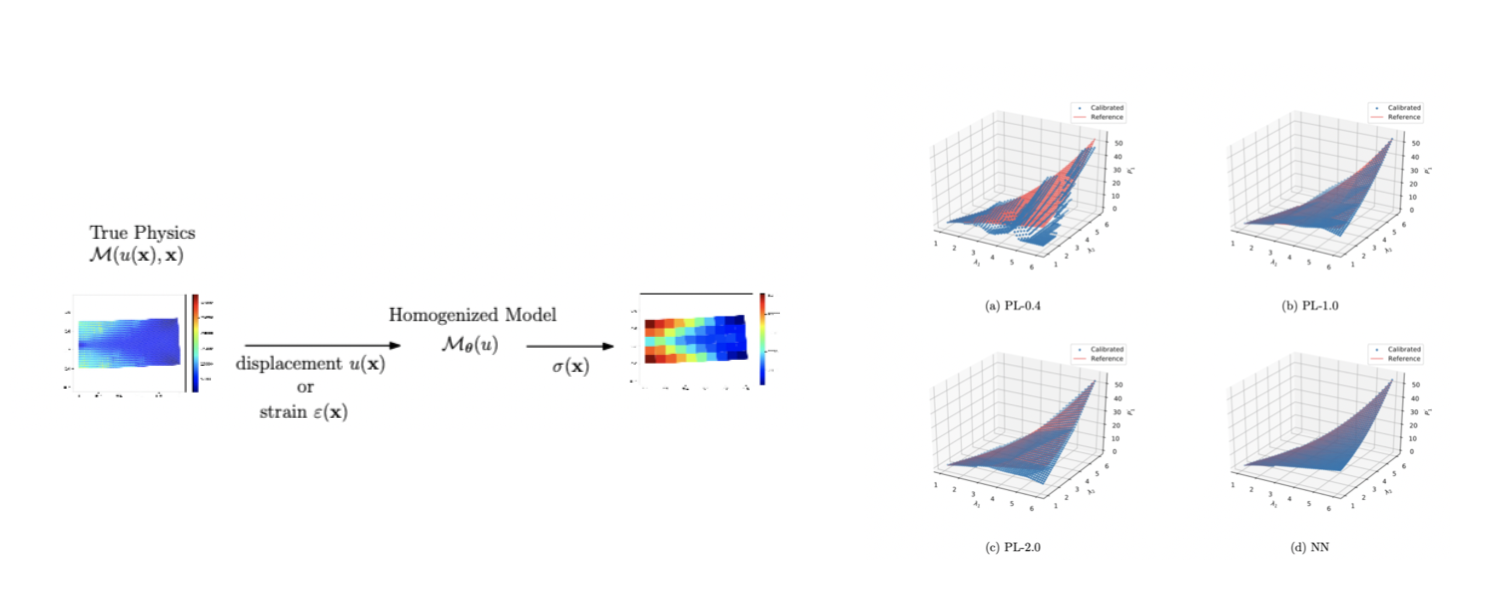
\includegraphics[width=1.0\textwidth]{../law.png}
\end{figure}
\end{frame}

\begin{frame}
	\frametitle{Probability Inverse Problem: Adversarial Numerical Analysis}
	
		\begin{equation*}
			\begin{cases}     -\nabla \cdot (a(x)\nabla u(x)) = 1 & x\in(0,1)\\
    u(0) = u(1) = 0 & \mbox{otherwise} \end{cases}
		\end{equation*}
		
		\begin{equation*}
			a(x) = 1-0.9\exp\left( -\frac{(x-\mu)^2}{2\sigma^2} \right)
		\end{equation*}

\begin{figure}[hbt]
	 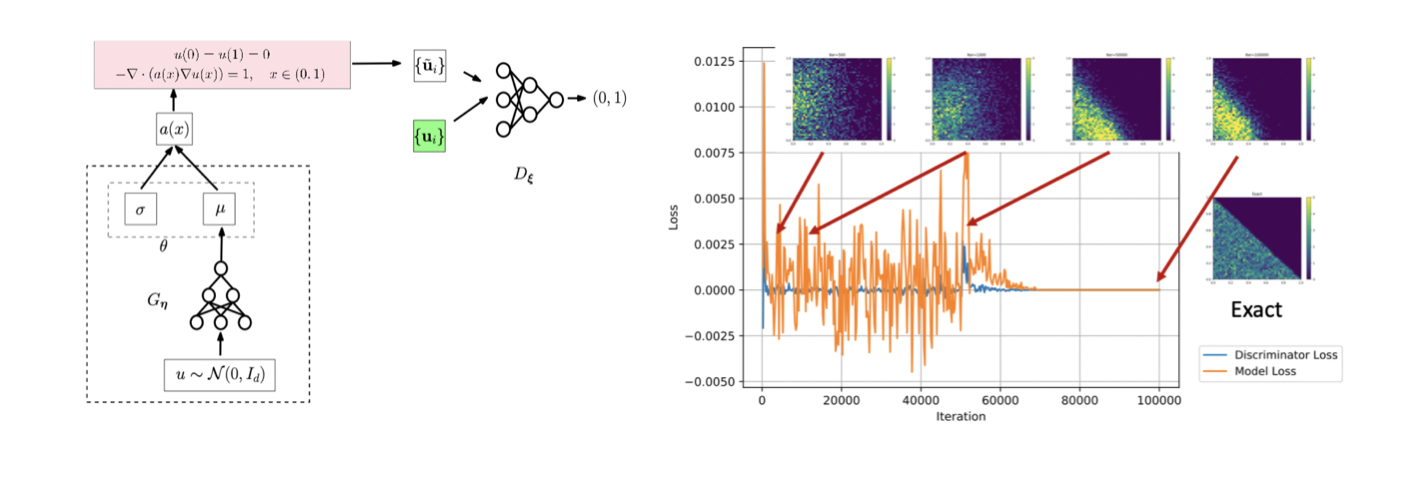
\includegraphics[width=1.0\textwidth]{../ana.png}
\end{figure}
\end{frame}

\begin{frame}
	\frametitle{A Cool Application: \texttt{ADSeismic.jl} (Coming soon)}
	\begin{itemize}
		\item An Open Source High Performance Package for General Seismic Inversion Problems
		\item Problems include:
		\begin{itemize}
		\item Full waveform inversion (FWI);
\item Rupture inversion;
\item Source-time inversion.
		\end{itemize}
		\item Features:
		\begin{itemize}
		\item (Multi-)GPU support;
		\item Easy-to-use;
		\item Easily extendable.
		\end{itemize}
	\end{itemize}
	
	\begin{figure}[hbt]
	 
\includegraphics[width=1.0\textwidth]{../adseismic.png}
\end{figure}
\end{frame}

%}
%\usebackgroundtemplate{}
%----------------------------------------------------------------------------------------
%    PRESENTATION SLIDES
%----------------------------------------------------------------------------------------

%------------------------------------------------



\end{document} 